\chapter{Ideation \& Specification}
\label{ch:ideation}
This chapter describes the ideation phase for a master thesis topic that aligns with the university's and Bosch Car Multimedia's interests' as well as my capabilities. The creative and brainstorming processes are guided by the Creative Technology design process \cite{Mader2014ATechnology}, which combines the concept of divergence and convergence with a cyclic concept. The chapter ends with the product specification.

\begin{figure}
    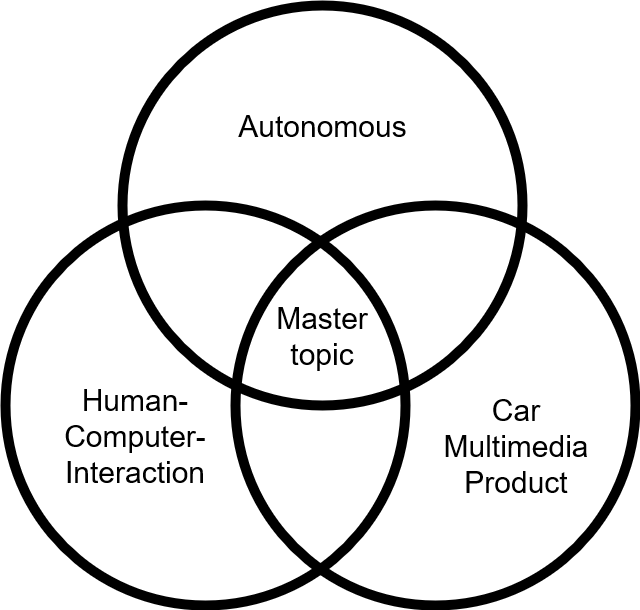
\includegraphics[height=0.4\textwidth]{fig/MasterTopic.png}
    \caption[Workshop]{The three topic ares for a master thesis topic}
    \label{fig:mastertopic}
\end{figure}

The University rejected the initial topic proposed by Robert Bosch Car Multimedia North America in Ann Arbour. The idea was to create a smell sensing device or algorithm that is capable of registering dirtiness in rental cars or autonomous vehicles. This topic hardly involves any interaction component or interaction design part. As Bosch did not have a topic alternative at hand, I developed the master topic on my own during the internship and worked on a few other tasks in parallel. The master topic should potentially result in a Car Multimedia Product, have a strong Human-Computer-Interaction component and should deal with autonomous vehicles (\emph{\fullref{fig:mastertopic}}). The Bosch Car Multimedia Division is currently making most of their money with infotainment systems, instrument clusters and head up displays. Infotainment Systems are the Software and Hardware that control the climate system, show the navigation system, control music, and radio or enable Apple CarPlay or Android Auto. The Instrument Cluster or head up displays show the speedometer, engine parameters, and navigation information. Fully autonomous vehicles, autonomous public vehicles, in particular, do not need any of these systems in their current form. In collaboration with an UX designer at Bosch, I discovered the frame of topics that would work for Bosch CM. Passenger to car interaction is of interest to Bosch Car Multimedia, but car to environment (pedestrians) interaction is not, as this would be the responsibility of another division. In the first steps, I created as many project ideas as possible and started to research if they were unique. I collected related works, concept ideas, used creative thinking methods and tinkering. Product ideas were sketched on paper, and a long topic list was compiled. 
\begin{figure}
    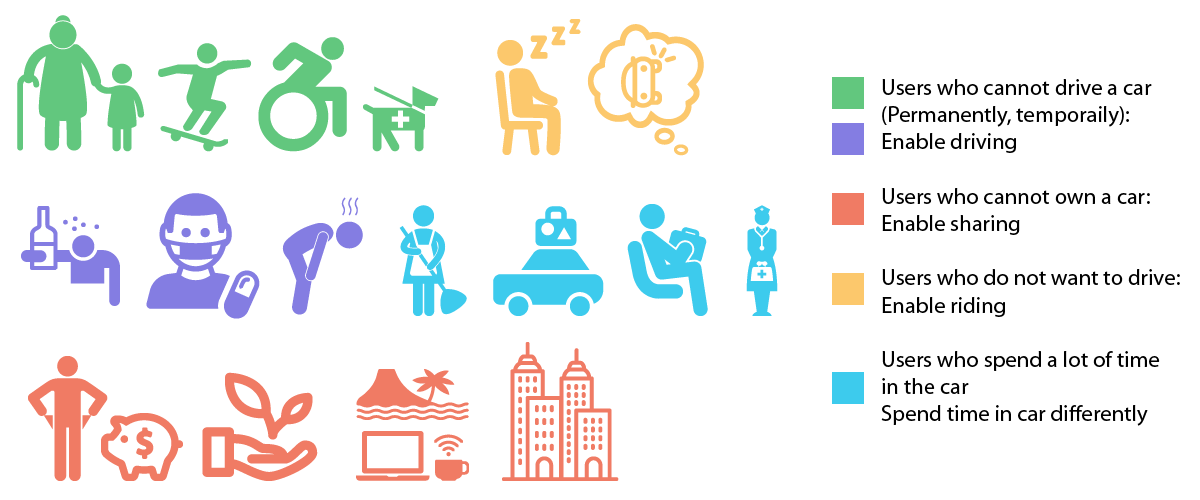
\includegraphics[width=1\textwidth]{fig/users.png}
    \caption[Users]{New user groups of autonomous vehicles: Elderly, young \& youth. Too sluggish \& too scared to drive. Drunk, sick \& tired. Workforce, travellers, commuters \& carers. Moneyless, savers, environmentally aware, nomads \& parking place restricted.}
    \label{fig:users}
\end{figure}

The seed for brainstorming was the newly reached user groups by autonomous vehicles (See  \emph{\fullref{fig:users}}) and the loss of human contact in cab scenarios. 

\emph{Cab driver tasks are:}
\begin{itemize*} 
  \item Clean \& maintain\quad
  \item Welcome (check tickets)\quad
  \item Help with luggage\quad
  \item Help with special needs\quad
  \item Plan route\quad
  \item Drive\quad
  \item Inform\quad
  \item Small-talk (personality)\quad
  \item Recommend (local)\quad
  \item Secure \& surveil (give trust)\quad
  \item Goodbye (pay)\quad
\end{itemize*}

Useful concepts for ideation were: Personalization \& context awareness, perceived intelligence of vehicle (personality and location of intelligence, possibility to express), shift from a ‘joy of driving’ to a ‘joy while driving’, living-room environment without using hands, cloud as a central hub where all information will pass through, shift from explicit to implicit interaction, discrepancy between public and private. Some HCI questions that need to be solved are: How can passengers feel that they are in control? How can passengers participate in driving decisions? How can the car talk, express and indicate? How does the car listen (direct \& passive)?

\begin{quotation}\emph{Starting with the user (blind, deaf, physical ability) to design an interior solution for autonomous cars during short duration (less than 15 minutes) commute. By basing this off the idea that if we design for a “disability” we, in turn, are designing for all. With your interactions with people who have different abilities you can uncover some of their needs and can redesign the interaction that this group has with a car. The solution could be voice, visual, or even haptic interactions. - Harsha, Bosch UX}\end{quotation}

In collaboration with the UX team, I turned these topic ideas into initial questions according to the Question Zero Concept from \cite{RobertBoschUX2017QuestionZero} and made sure that they align with the prioritization of activities (such as 'progressive vehicle interiors', NUIs and Mood Tech) according to the Bosch Mobility Trend Radar \cite{RobertBoschNA2017RegionalRegional}. 
Finally, the preferences of my supervisors at Bosch resulted in these topics:

    \begin{enumerate}
    \item Interior Communications through light.
    \item A system for an autonomous vehicle to communicate the driving decisions it takes to all passengers.
    \item Using voice as an interior control system.
    \item A product for visually or mentally impaired riders in autonomous vehicles that assures a sense of control when traveling alone.
    \item A system for passengers to gather trip information without the use of a driver.
    \item Other:
    \begin{itemize}
    \begin{sloppypar}
    \item A solution to reduce carsickness in autonomous vehicles.
     \item No located personal assistant but whole car interior as safe space (womb).
    \item Context-aware driving modes.
    \item Lowering distraction \& strengthening 
    the involvement of the driver through the use of V2V.
    \item Developing new usage scenarios/interactions for the BOSCH touch feedback system.
    \item A doorknob (window lifter etc.) which allows feeling in control in autonomous vehicles.
    \item Personality device (enable different car personalities for the use case, owner \& context).
    \end{sloppypar}
\end{itemize}
    \end{enumerate}

\section{Concept}
\label{sec:concept}
My personal interest is human-computer-interaction beyond screen-based interfaces. Concept cars from vehicle manufactures (\emph{\fullref{sec:conceptcars}}) rely heavily on large screens. Screens can be seen everywhere: In tables, windows, across the doors, behind the back seats, across the whole front and in the back of the seats. The best interface is no interface (\emph{\autoref{sec:nointerface}}). 

Almost in a 'flash of inspiration' the idea for the final product emerged: \emph{An indirectly illuminating LED bar that surrounds the whole cabin 360, and reaches all passengers with fluently distributed ambient information and mood lighting.} This light system should provide passengers with individual zone lightning that can be adjusted simply by touching it; enable the autonomous vehicles assistant to guide attention throughout the vehicle's cabin. Personal assistants such as Amazon Alexa and Google Assistant do not just rely on voice feedback but deepen the interaction through simple light feedback. This LED bar should be used to tell passengers crucial driving decisions the vehicle planned out and also allow it to communicate direction independently of the direction of travel: e.g., \say{Look over here for the empire state building}.
There is no driver to distract, therefore, brighter and more elaborate lightning can be used in cars. Fixed reading lights do not work with dynamic seating arrangements. Lightning can be used to calm or energize. Brought-ins (e.g., laptops, smartphones, game consoles and ebooks) will be the preferred entertainment and productivity tools over integrated infotainment systems. Car - passenger interaction is crucial, even if driving 'just works' without any interference by humans. 

\begin{figure}
    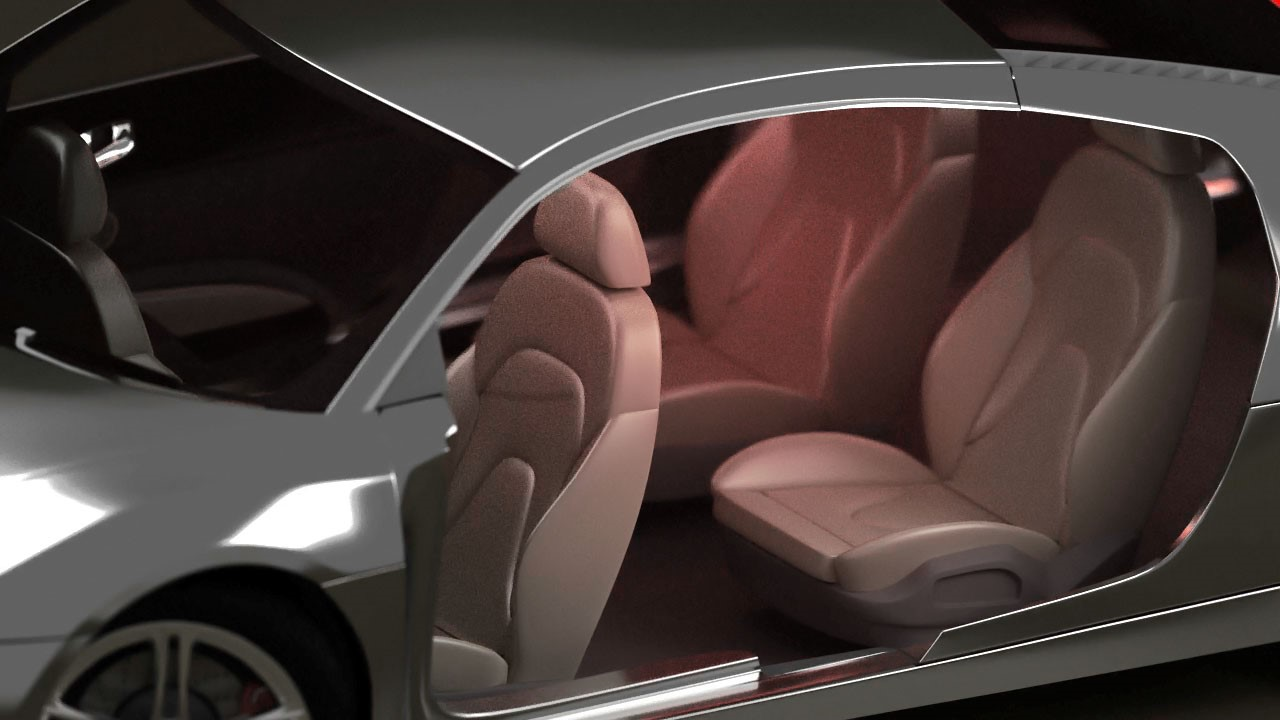
\includegraphics[height=0.28\textwidth]{fig/swerve_Mittel.jpg}\hfill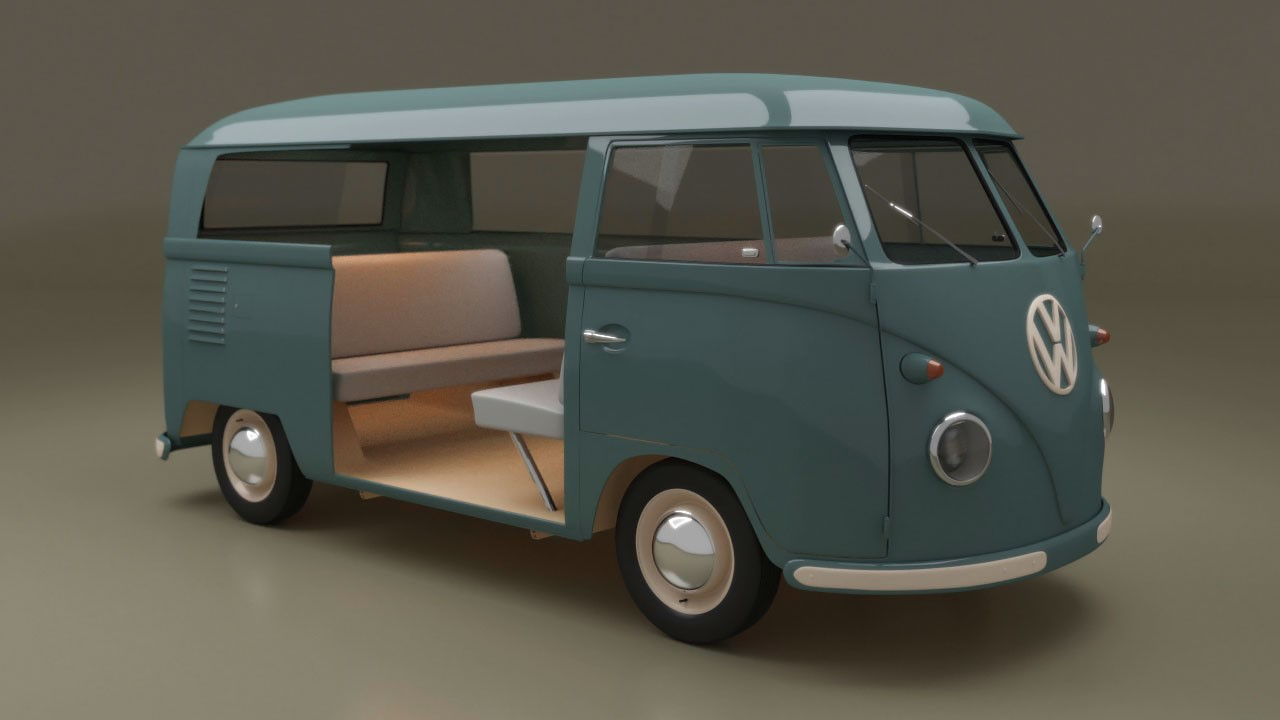
\includegraphics[height=0.28\textwidth]{fig/busLight_Mittel.jpg}\newline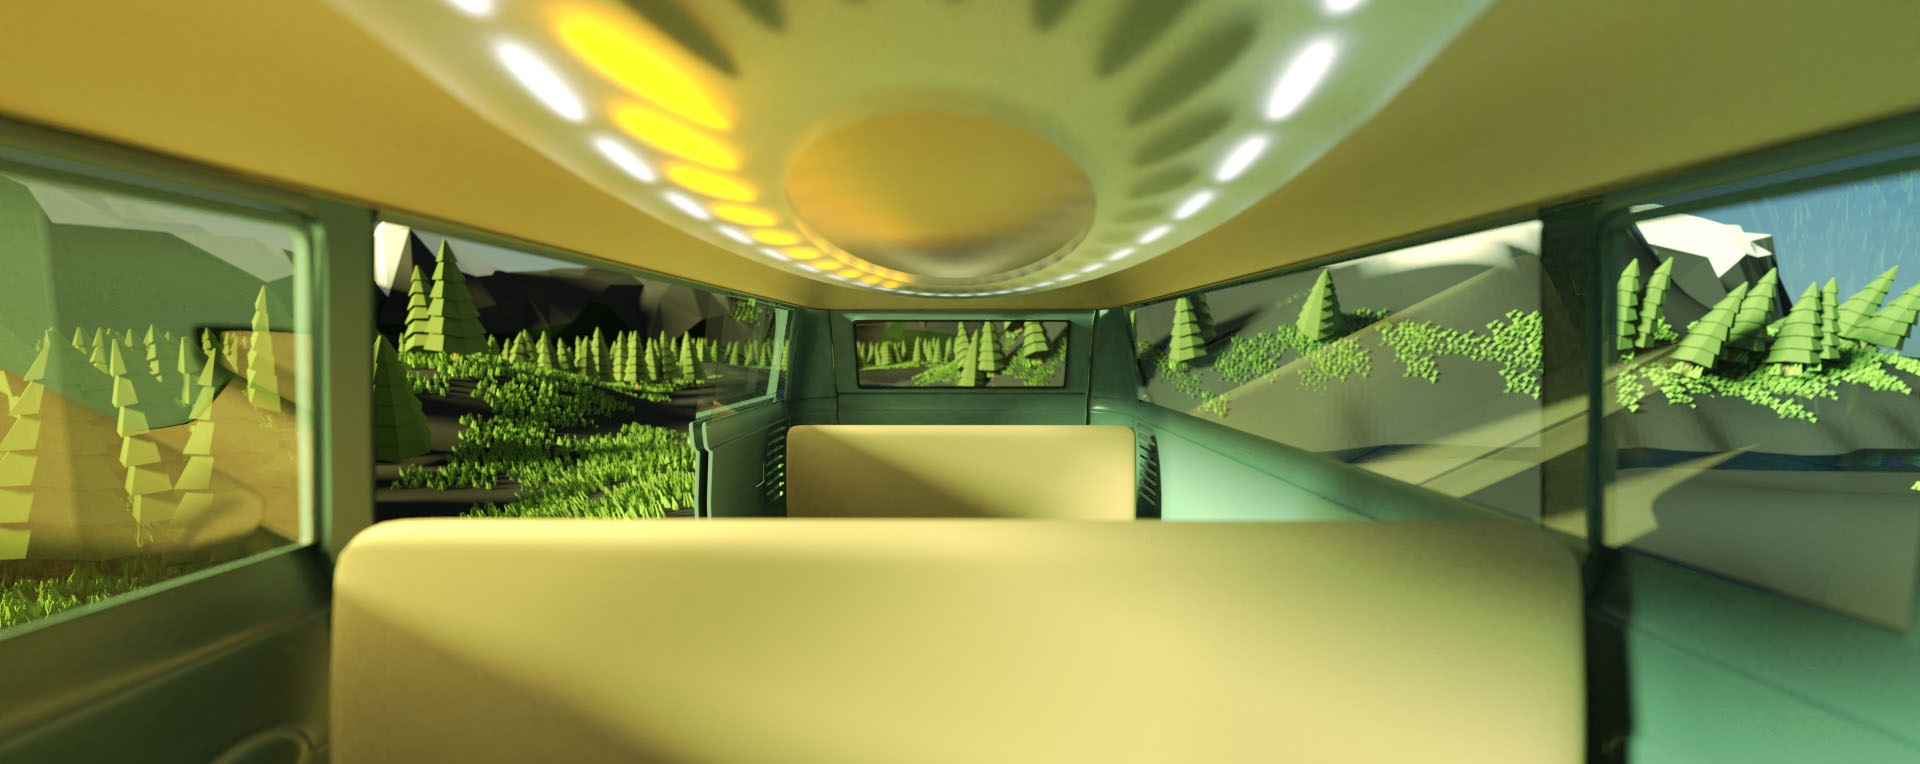
\includegraphics[width=1\textwidth]{fig/0013GRADIENTcut.jpg}
    \caption[Early Concept Render]{Early Concept Render: Swerve, Speed Up, Light Bar. (For animated versions check the digital appendix)}
    \label{fig:conceptrender}
\end{figure}

To convince supervisors of the potency of the concept and to try the feasibility of indirect lighting in vehicle cabins early on, looping GIF animations ( \emph{\fullref{fig:conceptrender}}) were rendered with the Blender Cycles renderer which provides global illumination through path tracing\footnote{\url{https://cglearn.codelight.eu/pub/computer-graphics/global-illumination}}. This allows visualizing indirect light and the light bounces inside the vehicle cabin. The 3D renderings use models that are licenced under creative commons license\footnote{\url{www.blendswap.com}: 1950's VW Van by Jay-Artist, Audi R8 V8 by Neubi, Mountain And River Low Poly by Hoboo}. The mood board in \emph{\autoref{fig:smoodboard}} contains visual and emotional inspiration for the project. It helps to set the atmosphere, communicate the idea of a finished product and the feelings it should provoke early on in the creative design process \cite{Cassidy2011TheTool}.

\begin{figure}
\centering
    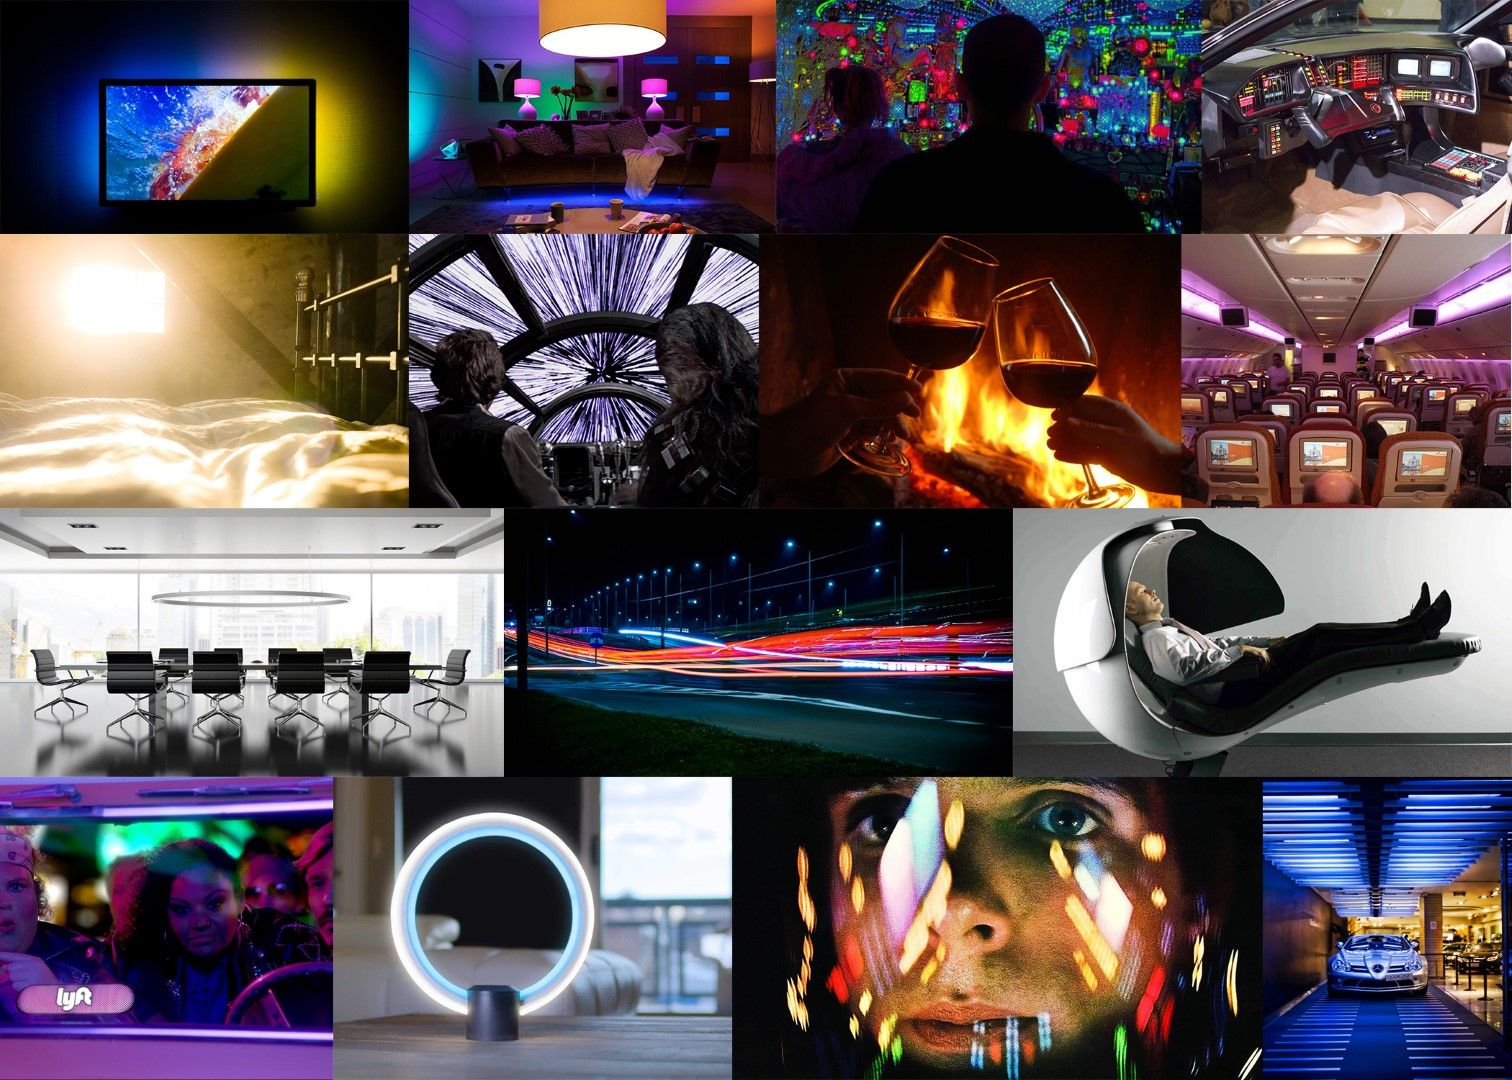
\includegraphics[width=1.\textwidth]{fig/moodboard_G.jpg}
    \caption[Moodboard]{Moodboard}
    \label{fig:smoodboard}
\end{figure}
\section{Light Animation Design}
\label{sec:Lightdesign}
In this section the design of light messages is discussed.

\subsection{Feedforward}
\label{ssec:feedforward}
Feedback in HCI is typically used to inform the user that the system is responding, to indicate progress or to confirm navigation. \citet{Djajadiningrat2002ButHow} state that feedforward, like feedback, returns information about the result of a process or activity. However, while feedback is communicated during or after the action, feedforward is information that is offered before the action takes place. Whereas feedback informs the user about the action that is carried out, feedforward informs the user about what the result of their action will be \citep{Vermeulen2013CrossingExecution}.

Feedforward is usually used in context with affordances of interfaces; here it is used as 'advance feedback before executing an action' \citep[see][]{Koo2015}. The automated machine provides this feedforward information irrespectively of user call for action. 
Feedforward is a new type of feedback that, in my opinion, should be provided by interactive automated systems to help humans understand their actions. 

\subsection{Message types}
The options for output in autonomous vehicles are almost endless. For multiple reasons, the users should not be overwhelmed with feedback from the vehicle. The low-resolution light display is limited by the number of different animations that can be displayed, the user cannot learn too many new messages at once and he might get annoyed by useless feedback. In a user study, we should only focus on a subset of messages to reduce complexity. Thereupon, it needs to be carefully curated what is considered important enough to be shown to the users.

In a driving context, it makes sense to distinguish between 'right now', 'soon' and 'planned long-term' information. ‘Right now’ is real-time information from the vehicle such as sensor data or outputs of the vehicle (driving). ‘Soon’ can be retrieved, e.g., from map data in the form of, e.g., calculated trajectories. Examples of planned long-term information are the route planning or traffic information. The light display might be best equipped to signal ‘right now’ and soon information because more complex future information is difficult to encode in such a ambient display and might be better suited for show through voice or displays. In the following scenarios that can be encoded by light animations are depicted. 

\subsubsection{Sudden driving behaviors}
Most of the sudden driving behaviors should only happen very rarely. Ideally, the autonomous vehicle is capable of foreseeing these scenarios early on and slow down smoothly. However, if they do happen the car should tell the passenger during these risky moves that it knows about the situation and is in control. Outside Vision is a light effect to show that other road users, who are driving recklessly, are noticed. (\emph{\fullref{fig:sudden}}). 
\begin{figure}
    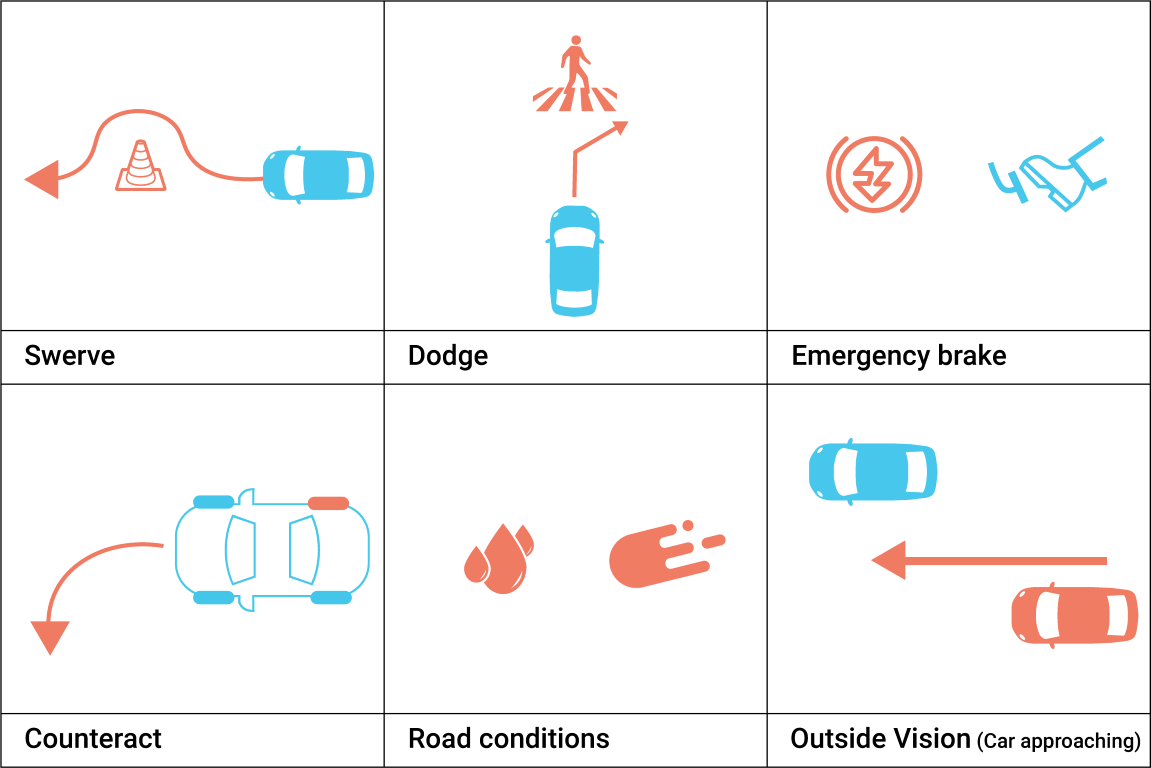
\includegraphics[width=1\textwidth]{fig/suddenmid.png}\hfill\
    \caption[Sudden Information]{Exemplary sudden information}
    \label{fig:sudden}
\end{figure}
\subsubsection{Planned}
Planned driving movements are most frequently shown. An autonomous vehicle or driver decides for these movements hundreds of times during driving. Even if the passengers can feel these movements with their body and deduce what the car is doing from how the street runs, the car should tell that is about to perform these actions. I hypothesize that the more noticeable these movements are, the more necessary it is to communicate them. Actions that are less frequent but deviate from the normal driving are more important to augment. (\emph{\fullref{fig:planned}}). 
\begin{figure}
    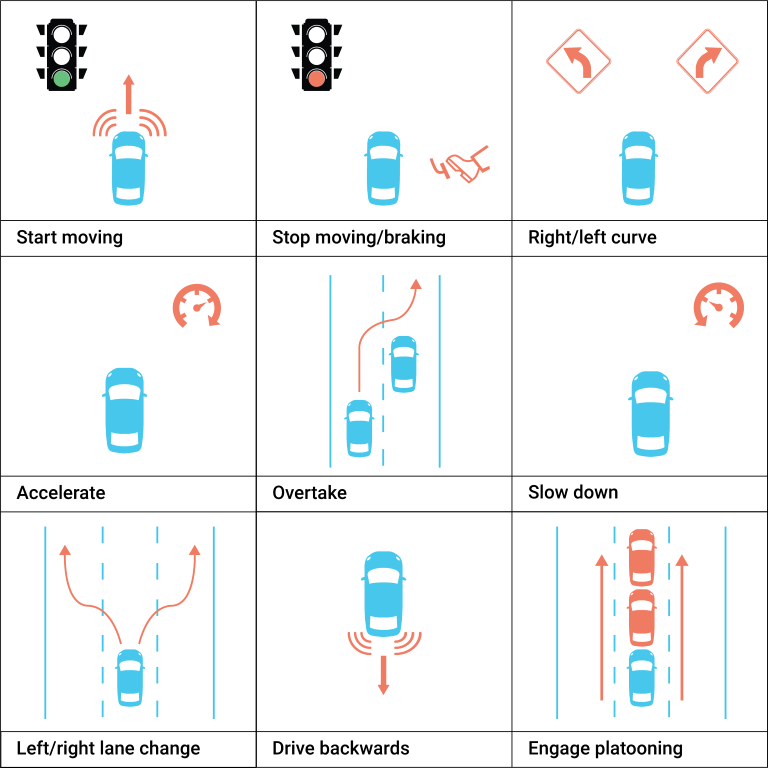
\includegraphics[width=1\textwidth]{fig/planned_1366.png}\hfill\
    \caption[Planned information]{Exemplary planned information}
    \label{fig:planned}
\end{figure}

\subsubsection{Route}
Route information is easily displayed through the navigation system of a car. Some of these pieces of information can be communicated actively by a light bar instead of passively by a display. Arrival time could be communicated by rising brightness; waking up the passengers and signaling that they have to become active again. Enter \& Exit can be animations that guide the passengers side of the car that it is safest to get off. Light signals can be used to draw attention to a specific direction. For example, a car could talk to the passengers about historical sights on the route and use light to show where to draw the attention (\emph{\fullref{fig:route}}). 
\begin{figure}
    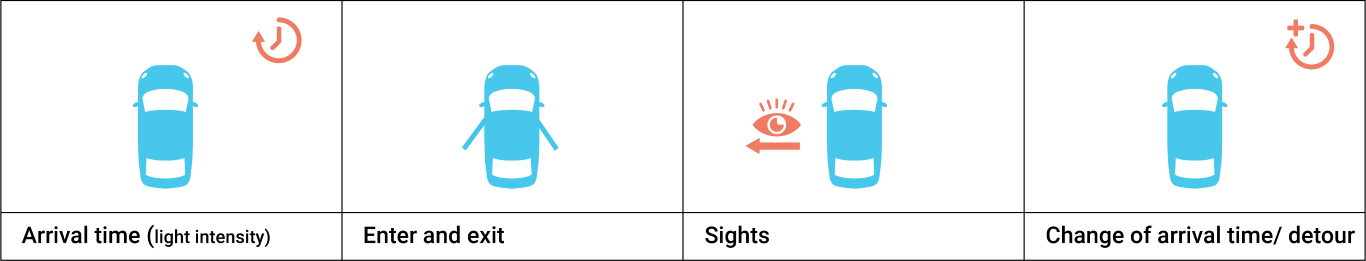
\includegraphics[width=1\textwidth]{fig/route.png}\hfill\
    \caption[Route information]{Exemplary route information}
    \label{fig:route}
\end{figure}

 In \emph{\fullref{fig:lightevents}} the messages are ordered by the underlying data and expected occurrence. Frequent events should be less notable, whereas exceptions must be strongly visible. States should not be too visible. Values can influence states and events but must not necessarily be visualized constantly. The subset of animations used in the final prototype was chosen according to their expected influence on driving comfort. 
 
\begin{figure}
    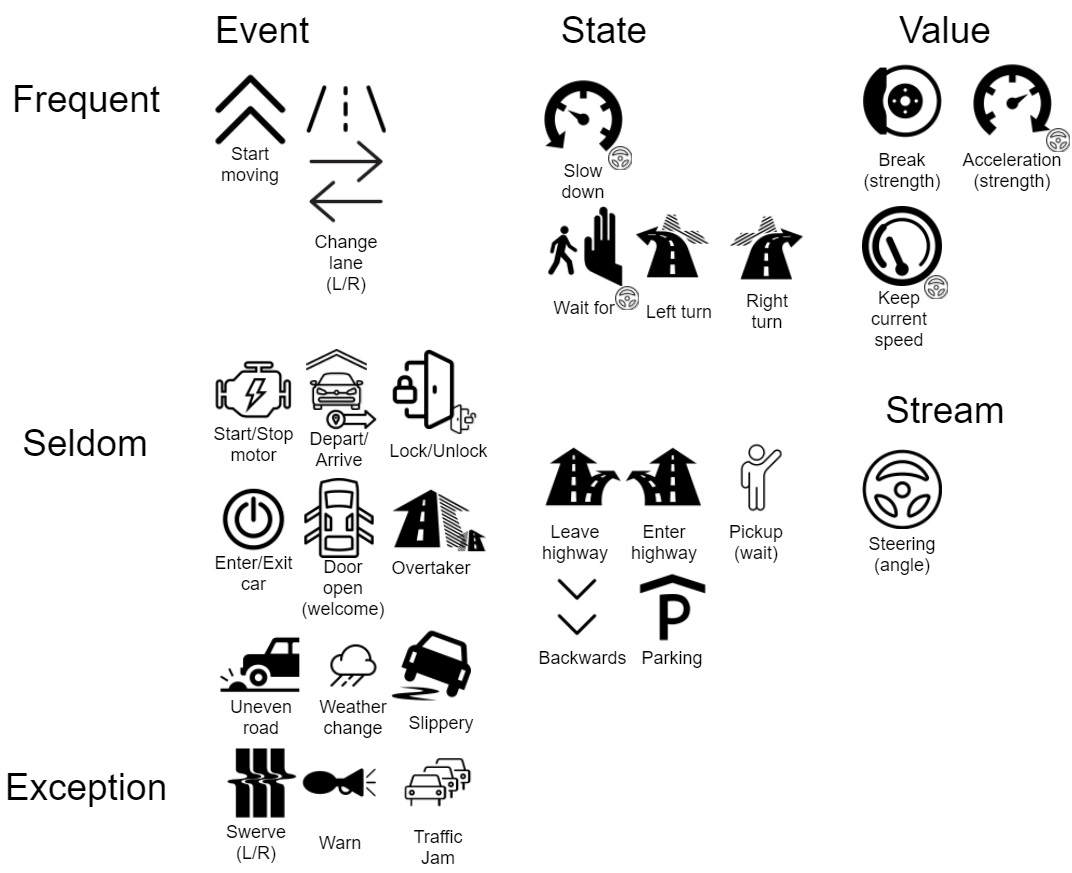
\includegraphics[width=\textwidth]{fig/tab-}
    \caption[Light Events]{Categorization of light messages by underling data}
    \label{fig:lightevents}
\end{figure}

\section{Animation behavior}
\begin{figure}
    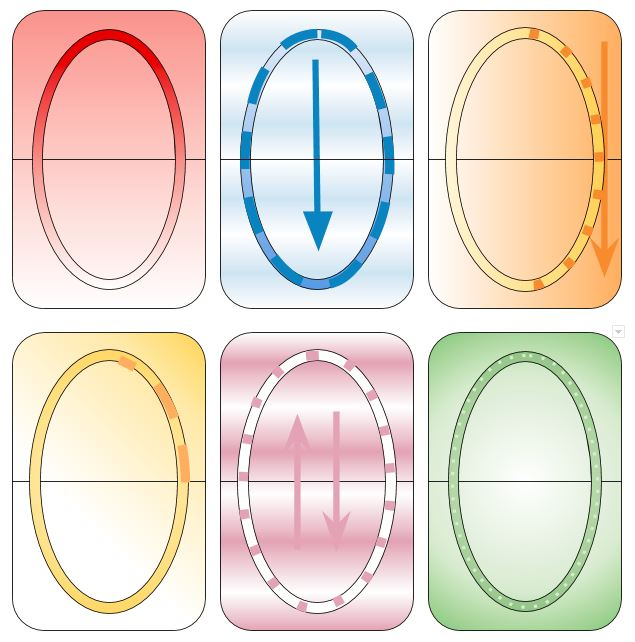
\includegraphics[width=0.6\textwidth]{fig/lightsignals.JPG}
    \caption[Light animations]{Graphical visualization of light animations. From top left to bottom right:
Brake (Hard), Accelerating, Into Right Lane, Right Turn, Uneven Road, Waiting}
    \label{fig:lightanimations}
\end{figure}
In \emph{\fullref{fig:lightanimations}} different ambient lighting animations are depicted. The arrows show the movement of animations, global 'fade in' and 'fade out' are not shown, the background gradients show how the car interior gets to light up. Brake and turn signal color coding is inspired by cues that the standard cars already give: red for brake lights and yellows for turn signals. This way signals that a car communicates to road users are projected inside the vehicle to passengers. Aggressive colors and colors that transport meaning by itself have to be used very carefully. Therefore, the red colors should not be too aggressive, e.g., for uneven road purple is used. 'Uneven road' uses forward and backward moving strips as a metaphor. A pulsating light depicts 'waiting' as if the car was in standby mode. Green could be interpreted as 'waiting for the green traffic light'. Accelerating is shown by fast moving blue lights, to give the impression of speed (See \emph{\fullref{fig:smoodboard}}).